\documentclass[../practica.root.tex]{subfiles}

\begin{document}
\section{Unidad 1}
\begin{enumerate}
    \item Representar graficamente las siguientes ecuaciones en $\R^3$
    % TODO: Encotrar una buena forma de graficar

    \item Demostrar que estas ecuaciones representan esferas

          \begin{enumerate}
              \item $x^2 + y^2 + z^2 - 6x + 4y - 2z = 11$
                    \[ x^2 - 6x + y^2 + 4y + z^2 - 2z = 11 \]
                    \[
                        x^2 - 6x + \left(\frac{6}{2}\right)^2
                        + y^2 + 4y + \left(\frac{4}{2}\right)^2
                        + z^2 - 2z + \left(\frac{2}{2}\right)^2
                        = 11
                        + \left(\frac{6}{2}\right)^2
                        + \left(\frac{4}{2}\right)^2
                        + \left(\frac{2}{2}\right)^2
                    \] \[
                        (x - 3)^2 + (y + 2)^2 + (z - 1)^2 = 11 + 3^2 + 2^2 + 1^2
                    \] \[
                        (x - 3)^2 + (y + 2)^2 + (z - 1)^2 = 25
                    \] \[
                        \boxed{C = (3,-2,1), r = \sqrt{25} = 5}
                    \]

              \item $4x^2 + 4y^2 + 4z^2 - 8x + 16y = 1$
                    \[ 4\left(x^2 + y^2 + z^2 - 2x + 4y = \frac{1}{4}\right) \]
                    \[ x^2 - 2x + y^2 + 4y + z^2 = \frac{1}{4} \]
                    \[
                        x^2 - 2x + \left(\frac{2}{2}\right)^2
                        + y^2 + 4y + \left(\frac{4}{2}\right)^2
                        + z^2
                        = \frac{1}{4}
                        + \left(\frac{2}{2}\right)^2
                        + \left(\frac{4}{2}\right)^2
                    \] \[
                        (x - 1)^2 + (y + 2)^2 + z^2 = \frac{1}{4} + 1 + 4
                    \] \[
                        (x - 1)^2 + (y + 2)^2 + z^2 = \frac{21}{4}
                    \] \[
                        \boxed{C = (1; -2; 0), r = \frac{\sqrt{21}}{2}}
                    \]
          \end{enumerate}

    \item Encontrar el componente vertical y horizontal. $\alpha = 38\deg$, $F = 50N$

          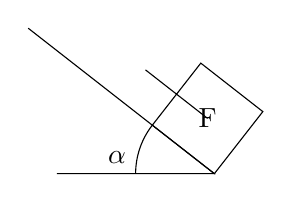
\begin{tikzpicture}[scale=2]
              \draw (-1,0) -- (0,0) -- (180-38:1.5);
              \draw (180-38:0.5) arc (180-38:180:0.5) node[anchor=south east]{$\alpha$};
              \draw[rotate=90-38] (0,0) rectangle (0.5,0.5) node[pos=0.5]{F} (0.25,0.25) -- +(0,0.5);
          \end{tikzpicture}
          \begin{align*}
              \cos\alpha \cdot F & = 39,4  \\
              \sin\alpha \cdot F & = 30,78 \\
          \end{align*}

    \item \dots

    \item Si $u \in \R^2$, hallar $u \cdot v$, $u \cdot w$.
          \begin{enumerate}
              \item
                    \begin{align*}
                        u \cdot v & = \left\| 1 \right\| \cdot \left\| 1 \right\| \cos(120 \deg) = \boxed{-0,5} \\
                        u \cdot w & = \left\| 1 \right\| \cdot \left\| 1 \right\| \cos(120 \deg) = \boxed{-0,5} \\
                    \end{align*}
              \item
                    \[ \|v\| = \sqrt{2\|u\|^2}/2 = \frac{\sqrt{2}}{2}  \]
                    \begin{align*}
                        u \cdot v & = \frac{\sqrt{2}}{2}\cdot \cos(-45\deg) = \frac{\sqrt{2}}{2}\cdot\frac{1}{\sqrt{2}} = \boxed{0,5} \\
                        u \cdot w & = \boxed{0}                                                                                       \\
                    \end{align*}

          \end{enumerate}

    \item Hallar $p_u(v)$
          \[ p_u(v) = \frac{uv}{\|u\|^2}u \]
          \begin{enumerate}
              \item  \dots
                    \[ \frac{(3;-4)(5;0)}{\|(3;-4)\|^2}(3;-4) \]
                    \[ \frac{15}{25}(3;-4) = \frac{3}{5}(3;-4) \]
                    \[ \boxed{\left(\frac{9}{5}; -\frac{3}{5}\right)} \]
              \item  \dots
              \item  \dots
              \item  \dots
          \end{enumerate}

    \item Mostrar $v - p_u(v)$ es ortogonal a $u$
          \begin{proof}
              \[ \left(v - u\frac{uv}{\|u\|^2}\right)\cdot u = 0 \]
              \[ uv - uu\frac{uv}{\|u\|^2} = 0 \]
              \[ uv - \|u\|^2\frac{uv}{\|u\|^2} = 0 \]
              \[ uv - uv = 0 \]
          \end{proof}

    \item Encotrar $p_u(v) = p_v(u)$
          \begin{proof}
              \[ \frac{uv}{\|u\|^2}u = \frac{vu}{\|v\|^2}v \]
              \[ \frac{uuv}{\|u\|^2} = \frac{vvu}{\|v\|^2} \]
              \[ \frac{\|u\|^2v}{\|u\|^2} = \frac{\|v\|^2u}{\|v\|^2} \]
              \[ v = u \]
          \end{proof}

    \item
          \[ W = 4 \cdot \SI{20}{\newton} \cdot \cos(\SI{50}{\degree}) = \boxed{\SI{51,42}{\joule}}  \]

    \item  $P = (0; 10; 8)$, $Q = (6; 12; 20)$ y $F = (8; -6; 9)$
          \[ (Q - P)\cdot F = (6; 2; 12)\cdot(8; -6; 9) = \boxed{142} \]

    \item Calcular $u \x v$ y $\|u \x v\|$
          \[ \|u \x v\| = \|u\|\|v\|\sen\theta \]
          \begin{enumerate}
              \item
                    \begin{tikzpicture}[scale = 0.5]
                        \draw[style=vec] (0,0) -- (90:5) node[pos=0.5,anchor=east] {$\|u\| = 5$};
                        \draw[style=vec] (0,0) -- (30:10) node[pos=0.5,anchor=north west] {$\|v\| = 10$};
                        \draw (30:1) arc (30:90:1) node[pos=0.5, anchor=south west,rotate=30] {$\theta =  \SI{60}{\degree}$};
                    \end{tikzpicture}
                    \[ \|u \x v\| = 5*10*\frac{\sqrt{3}}{2} = \boxed{25\sqrt{3}} \]
              \item
                    \begin{tikzpicture}[scale = 0.5]
                        \draw[style=vec] (-6,0) -- (0,0)  node[pos=0.5,anchor=south] {$\|u\| = 6$};
                        \draw[style=vec] (0,0) -- (-30:8) node[pos=0.5,anchor=south west] {$\|v\| = 8$};
                        \draw (-30:1) arc (-30:-180:1) node[pos=0.5,anchor=north] {$\theta = \SI{150}{\degree}$};
                    \end{tikzpicture}
                    \[ \|u \x v\| = 6*8*\frac{1}{2} = \boxed{24} \]

          \end{enumerate}

    \item Calcular el area del paralelogramo de $A = (1; 2; 3)$, $B = (1; 3; 6)$, $C = (3; 8; 6)$, $D = (3; 7 ;3)$ \\
          Verificar que los 4 vectores formen un paralelogramo. (Uno tiene que ser l. d. del resto) \\
          \[
              \begin{pmatrix}
                  1 & 2 & 3 \\
                  1 & 3 & 6 \\
                  3 & 8 & 6 \\
                  3 & 7 & 3
              \end{pmatrix}
              \equiv
              \begin{pmatrix}
                  1 & 0 & 0 \\
                  0 & 0 & 1 \\
                  0 & 0 & 0 \\
                  0 & 1 & 0
              \end{pmatrix}
          \]
          \[
              \|(B-A)\x(C-A)\| = \|(0; 1; 3)\x(2; 6; 3)\| = \|(-15; 6; -2)\|
          \] \[
              \sqrt{(-15)^2 + 6^2 + (-2)^2} = \sqrt{225 + 36 + 4} = \boxed{2\sqrt{74}}
          \]

    \item \dots
          \[F \cdot P = \SI{60}{\newton}\SI{0,18}{\m}\sen(80º) = \boxed{\SI{10,6}{\joule}} \]

    \item Sea $u,v,w \in \R^3$
          \[
              \left\|
              \begin{pmatrix}
                  u_1 & u_2 & u_3 \\
                  v_1 & v_2 & v_3 \\
                  w_1 & w_2 & w_3 \\
              \end{pmatrix}
              \right\|
              =
              \begin{array}{rl}
                  -u_3 v_2 w_1  & + u_2 v_3 w_1 \\
                  + u_3 v_1 w_2 & - u_1 v_3 w_2 \\
                  - u_2 v_1 w_3 & + u_1 v_2 w_3
              \end{array}
              =
              \begin{array}{rl}
                  - u_1 v_3 w_2 & + u_1 v_2 w_3 \\
                  - u_2 v_1 w_3 & + u_2 v_3 w_1 \\
                  + u_3 v_1 w_2 & -u_3 v_2 w_1
              \end{array}
          \] \[
              =
              \begin{array}{rl}
                  u_1(- v_3 w_2   & + v_2 w_3) \\
                  + u_2(- v_1 w_3 & + v_3 w_1) \\
                  + u_3(+ v_1 w_2 & -v_2 w_1)
              \end{array}
          \] \[
              u \cdot (v \x w) = (u_1; u_2; u_3) \cdot (-v_3w_2+v_2w_3; -v_1w_3+v_3w_1; v_1w_2-v_2w_1)
          \] \[
              (v \x w) = (-v_3w_2+v_2w_3; -v_1w_3+v_3w_1; v_1w_2-v_2w_1)
          \]

    \item Con $A = (2; 0; -1)$, $B = (4; 1; 0)$, $C = (3; -1; 1)$ y $D = (2; -2; 2)$,
          calcular el volumen del paralelepípedo con lados $AB$, $AC$ y $AD$

          \begin{tikzpicture}[tdplot_main_coords,grid/.style={very thin,gray},axis/.style={->,blue,thick}]
              \coordinate (O) at (0, 0, 0);
              \coordinate (A) at (2, 0, 1);
              \coordinate (B) at (4, 1, 0);
              \coordinate (C) at (3, -1, 1);
              \coordinate (D) at (2, -2, 2);

              \foreach \x in {0,1,2,3,4}
              \foreach \y in {0,1,2,3,4}
                  {
                      \draw[grid] (\x,0) -- (\x,4);
                      \draw[grid] (0,\y) -- (4,\y);
                  }
              \draw[axis] (0,0,0) -- (3,0,0) node[anchor=west]{$x$};
              \draw[axis] (0,0,0) -- (0,3,0) node[anchor=west]{$y$};
              \draw[axis] (0,0,0) -- (0,0,3) node[anchor=west]{$z$};

              \draw (A) node {$A$};
              \draw (B) node {$B$};
              \draw (C) node {$C$};
              \draw (D) node {$D$};

              \draw (A) -- (B) -- ++(C) -- ++(D);
              \draw (A) -- (C) -- ++(D) -- ++(B);
              \draw (A) -- (D) -- ++(C) -- ++(B);
          \end{tikzpicture}
          \[ | ((B-A)\x(C-A))\cdot(D-A) | \]
          \[ u = B - A, v = C - A, w = D - A \]
          \[ v\x w = (1; -3; -2) \]
          \[ | u(v \x w) | = \boxed{3} \]

    \item Decidir si $A = (1;3;2)$, $B = (3;-1;6)$, $C = (5;2;0)$, $D = (3;6;-4)$ están en el mismo plano
          \[ N = (A-C) \x (B-C) = (-4;1;2) \x (-2;-3;6) = (12;20;14) \]
          \[ \Pi: 12x - 20y + 14z = d \]
          \[ d = N \cdot C = 100 \]
          \[ \Pi: 12x - 20y + 14z = 100 \]
          Probar $D \in \Pi$
          \[ 12*3 - 20*6 + 14*(-4) = 100 \]
          \[ -140 \neq 100 \]
          \[ \boxed{\text{$D$ no pertenece al plano formado por $A$, $B$ y $C$}} \]


    \item \dots
    \item \dots


\end{enumerate}
\end{document}
